\documentclass[8pt]{article}
\usepackage{natbib}
\usepackage{hyperref}
\usepackage{graphicx}
\usepackage{amsmath}
\usepackage{fullpage}
\usepackage[FIGTOPCAP]{subfigure}
\usepackage{fancyvrb}
\usepackage[utf8]{inputenc}
\usepackage{helvet}
\renewcommand{\familydefault}{\sfdefault}

\begin{document}

\pagenumbering{gobble}

\begin{figure}[h]
	\begin{center}
		\renewcommand\thesubfigure{(A)}
    	\subfigure[Mean batch effect estimates within each sample]{
    		\renewcommand\thesubfigure{}
    		\subfigure[No Adjustment]{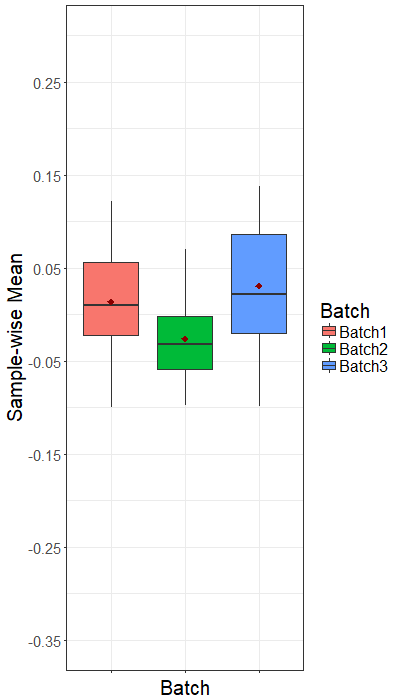
\includegraphics[width=0.25\textwidth]{scaledSig_sampleMean_box_Original.png}} 
    		\subfigure[Mean-only ComBat]{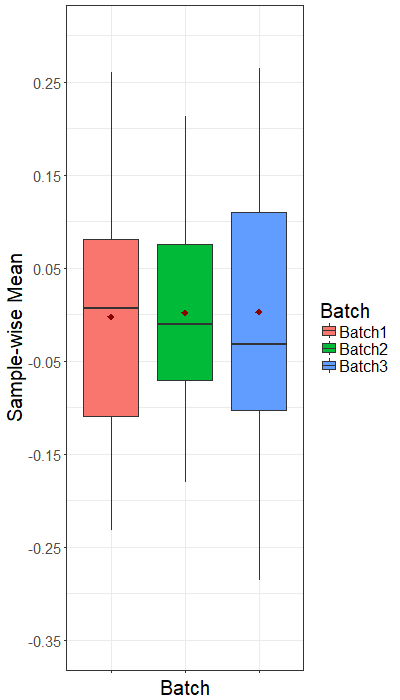
\includegraphics[width=0.25\textwidth]{scaledSig_sampleMean_box_Meanonly.png}} 
   	 		\subfigure[Mean/variance ComBat]{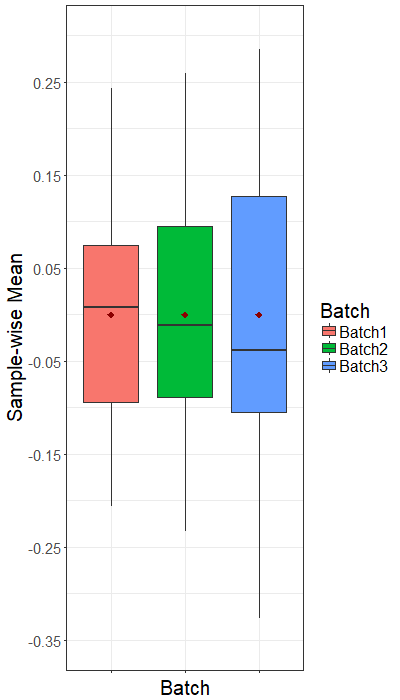
\includegraphics[width=0.25\textwidth]{scaledSig_sampleMean_box_ComBat.png}}
   	 	}  \\
   	 	\renewcommand\thesubfigure{(B)}
   	 	\subfigure[Variance batch effect estimates within each sample]{
   	 		\renewcommand\thesubfigure{}
    		\subfigure[No Adjustment]{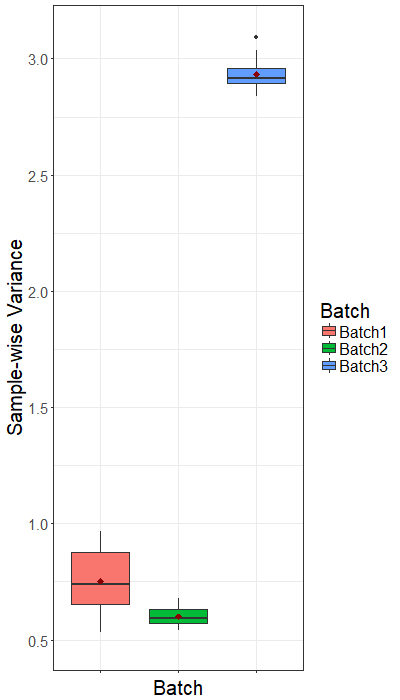
\includegraphics[width=0.25\textwidth]{scaledSig_sampleVariance_box_Original.png}} 
    		\subfigure[Mean-only ComBat]{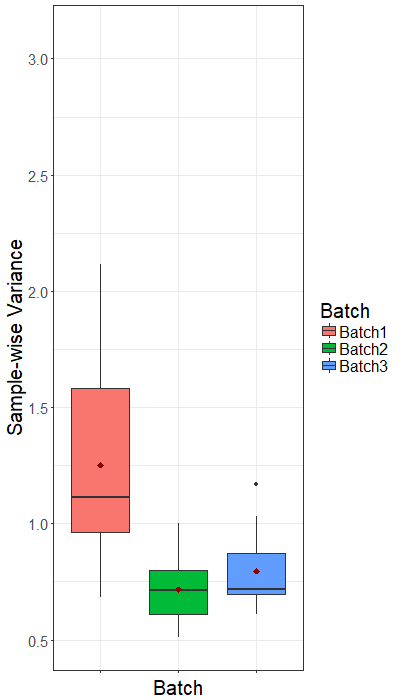
\includegraphics[width=0.25\textwidth]{scaledSig_sampleVariance_box_Meanonly.png}} 
   	 		\subfigure[Mean/variance ComBat]{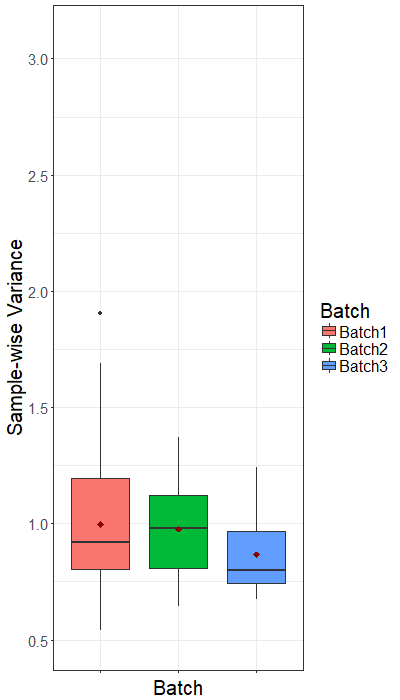
\includegraphics[width=0.25\textwidth]{scaledSig_sampleVariance_box_ComBat.png}}
   	 	}
  	\end{center}
\end{figure}

\end{document}